\section{Procedure}
The experiment can be divided into two parts: first, the examination of various 
amplitude gratings, and second, the measurement of a phase modulating grating, 
thus the introduction into acousto-optics. The single steps are the following:
\begin{enumerate}
    \item
        Calibration and establishing the relationship between difference in time 
        read off the oscilloscope and distance between the corresponding maxima, 
        using a gauge grating.
    \item
        Examination of amplitude gratings, consisting of the following steps:
        \begin{enumerate}
            \item
                Measuring a sine amplitude grating and determining the distance of the first 
                order maximum.
            \item
                Determination of lattice costant and resolution of five amplitude gratings.
            \item
                Calculation of aperture function and further 
                determination of the ratio of slitwidth and grating constant of the first grating. 
        \end{enumerate}
        \item
            Examination of the phase grating induced by an ultrasonic wave. 
            This part consists of the following tasks:
        \begin{enumerate}
            \item
                Measuring the intensity distribution for different voltages applied to the cell;
            \item
                Comparing the results to Raman-Naht theory;
            \item
                Determination of wave length of the ultrasonic wave.
        \end{enumerate}
\end{enumerate}

\section{Experimental setup}
The setup of the entire experiment is contained in one beam path. 
For the different parts of the experiment, the gratings or the tank 
filled with isooctan (referred to as the "ultrasonic cell") will be 
taken out or installed as necessary. An overview is given in figure \ref{fig:setup}

\begin{figure}
    \centering
    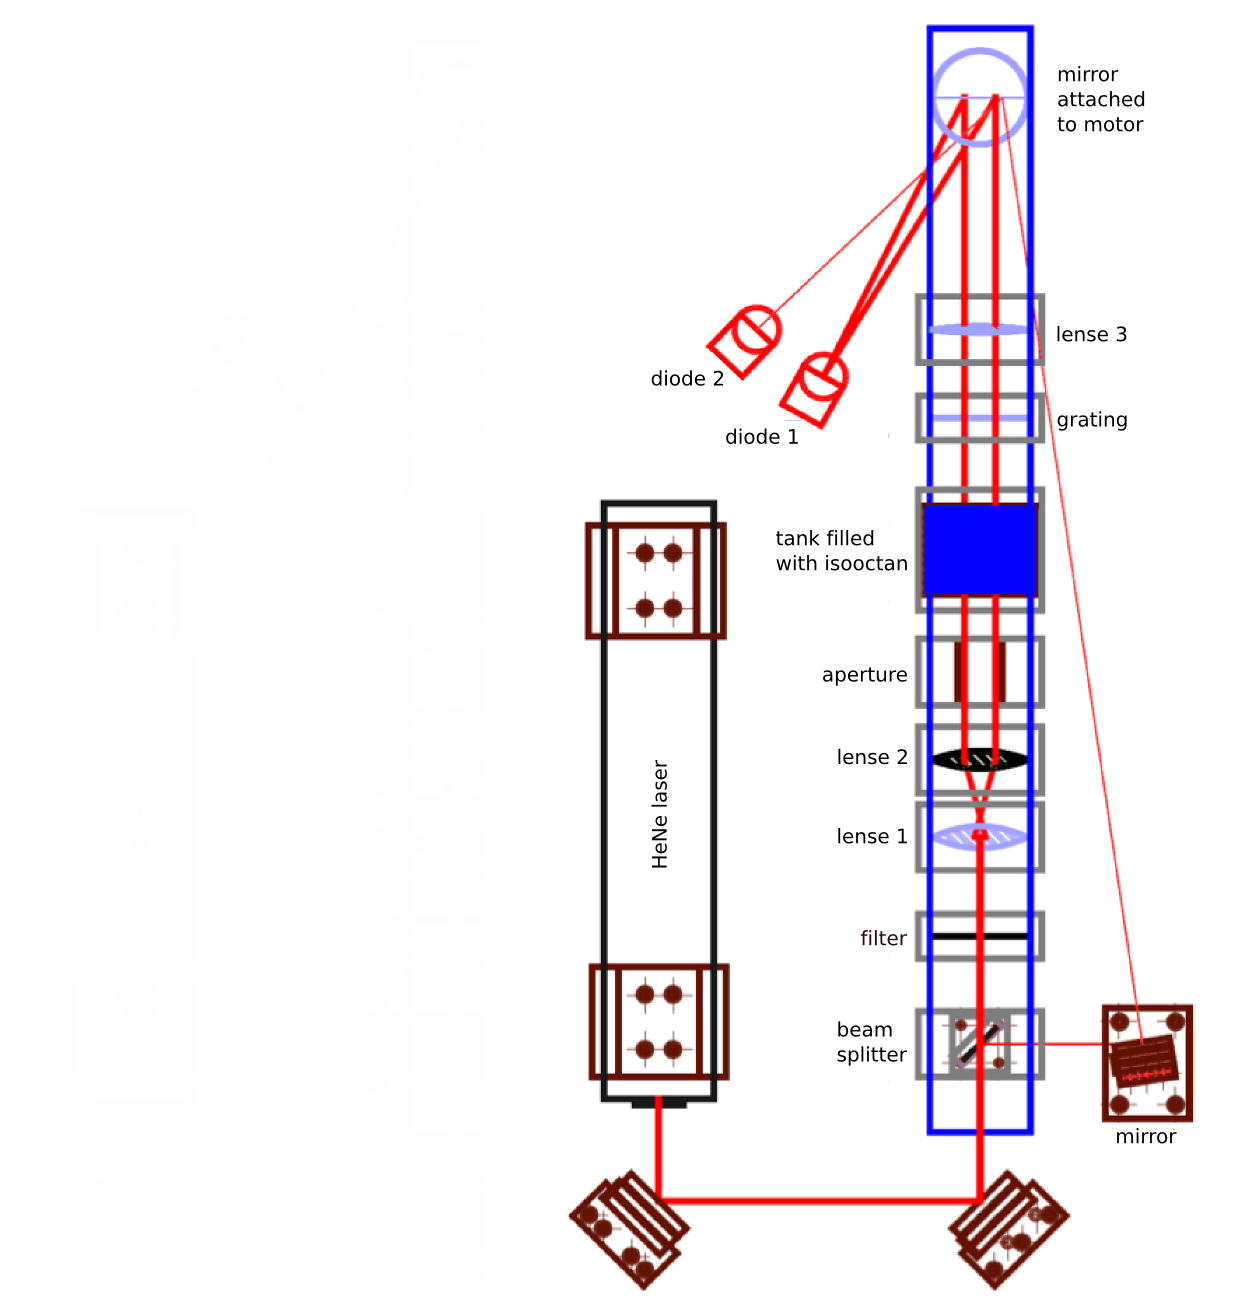
\includegraphics[width=1.0\textwidth]{figures/setup_bitmap.png}
    \caption{
        Scheme of the experimental setup. The tank or the gratings will be taken out 
        according to each part of the experiment.
        Modified, from \cite{ver}.
        }
    \label{fig:setup}
\end{figure}
